%%%%%%%%%%%%%%%%%%%%%%%%%%%%%%%%%%%%%%%%%%%%%%%%%%%%%%%%%%%%%%%%%%%%%%%%%%%%%
%
%  System        : 
%  Module        : 
%  Object Name   : $RCSfile$
%  Revision      : $Revision$
%  Date          : $Date$
%  Author        : $Author$
%  Created By    : Robert Heller
%  Created       : Sat Apr 15 10:38:55 2023
%  Last Modified : <230422.1645>
%
%  Description 
%
%  Notes
%
%  History
% 
%%%%%%%%%%%%%%%%%%%%%%%%%%%%%%%%%%%%%%%%%%%%%%%%%%%%%%%%%%%%%%%%%%%%%%%%%%%%%
%
%    Copyright (C) 2023  Robert Heller D/B/A Deepwoods Software
%			51 Locke Hill Road
%			Wendell, MA 01379-9728
%
%    This program is free software; you can redistribute it and/or modify
%    it under the terms of the GNU General Public License as published by
%    the Free Software Foundation; either version 2 of the License, or
%    (at your option) any later version.
%
%    This program is distributed in the hope that it will be useful,
%    but WITHOUT ANY WARRANTY; without even the implied warranty of
%    MERCHANTABILITY or FITNESS FOR A PARTICULAR PURPOSE.  See the
%    GNU General Public License for more details.
%
%    You should have received a copy of the GNU General Public License
%    along with this program; if not, write to the Free Software
%    Foundation, Inc., 675 Mass Ave, Cambridge, MA 02139, USA.
%
% 
%
%%%%%%%%%%%%%%%%%%%%%%%%%%%%%%%%%%%%%%%%%%%%%%%%%%%%%%%%%%%%%%%%%%%%%%%%%%%%%

\subsection{Automatic Block Signals}
\label{sect-appl:ABS}

\begin{figure}[hbpt]\begin{centering}%
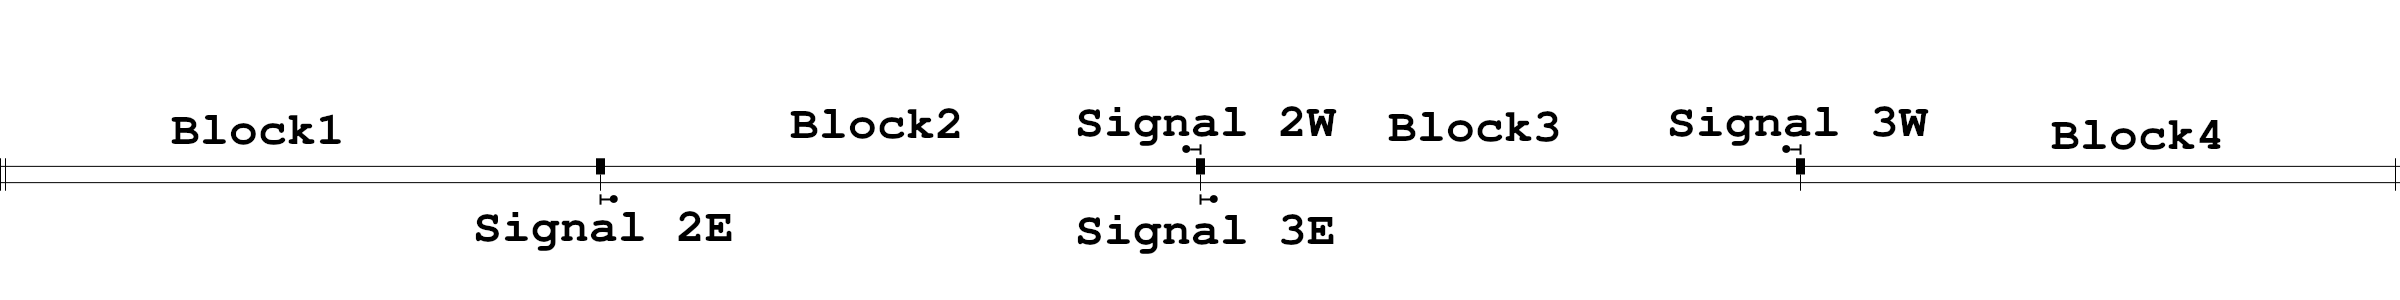
\includegraphics[width=5in]{ABSTrack.png}
\caption{Automatic Block Signaled track.}
\label{fig:ABSTrack}
\end{centering}\end{figure}

Figure~\ref{fig:ABSTrack} is a simple bi-directional segment of ABS signaled 
track, with four blocks and four signals, wired to a node as follows:

\begin{description}
\item [OC 1] Block 1
\item [OC 2] Block 2
\item [OC 3] Block 3
\item [OC 4] Block 4
\item [A0(R), A1(Y), A2(G)] Signal 2E
\item [A3(R), A4(Y), A5(G)] Signal 3E
\item [B0(R), B1(Y), B2(G)] Signal 2W
\item [B3(R), B4(Y), B5(G)] Signal 3W
\end{description}

Each signal will use three Logic elements:

\begin{enumerate}
\item Will be triggered true if the block is occupied and will select the Stop 
rule.
\item Will be triggered true if the next signal mast is stop (via a track 
circuit) and will select the Approach rule.
\item Will always be true and will select the Clear rule.
\end{enumerate}

\begin{figure}[hbpt]\begin{centering}%
\includegraphics[width=5in]{ABSTrack_EventID.pdf}
\caption{ABSTrack Event Id graph.}
\label{fig:ABSTrackEventID}
\end{centering}\end{figure}
\begin{table}[hbpt]\begin{centering}%
\begin{tabular}{|l|l|p{2in}|}
\hline
Color&Object&What it is\\
\hline
Orange&Node&Occupancy Detectors\\
\hline
Cyan&Node&Logic Elements\\
\hline
RoyalBlue&Node&Masts\\
\hline 
Black&Edge&Logic Fallthroughs (Elses)\\
\hline
Cyan&Edge&Mast Rule Selection\\
\hline
\end{tabular}
\caption{Graph color key}
\label{tab:ExampleSidingCP1EventFlow}
\end{centering}\end{table}
                                        
